%%%%%%%%%%%%%%%%%%%%%%%%%%%%%%%%%%%%%%%%%%%%%%%%%%
%\subsection{Education and Future Wages}\label{subsec:card}

%Note: For more information, see the original article:
% David Card,
%"Using Geographic Variation in College Proximity to Estimate the Return to Schooling"
% NBER Working Paper 4832, August 1994
%
%This article is published (with the same title and identical tables)
%in  Aspects of Labour Market Behaviour: Essays in Honour of John Vandekamp"
%edited by Louis N. Christofides, E. Kenneth Grant, and Robert Swidinsky
%Toronto: University of Toronto Press, 1995.
%
%The file contains 3613 observations on men in 1976 cross-section
%of nls young men (original nls cohort)

%y = card$ed76
%x = cbind(card$nearc2,card$nearc4,card$exp76,card$exp762,card$black,card$smsa76r,card$reg76r)
%xnms = c("nearc2","nearc4","exp76","exp762","black","smsa76r","reg76r")

%ed76  /*educ in 1976*/
% 7 -  7     nearc2  /*grew up near 2-yr college*/
%10 - 10     nearc4  /*grew up near 4-yr college*/

%     114 -114     black  /* 1 if black*/
%     116 -116     smsa76r /*in smsa in 1976*/
%     118 -118     smsa78r /*in smsa in 1978*/
%     120 -120     reg76r /*in south in 1976*/

%> dim(card)
%[1] 3613   53
%> subset = which(!is.na(card$lwage76))
%> card = card[subset,]
%> dim(card)
%[1] 3010   53

%Card (1995) considers the time honored question of the returns to education, exploiting geographic
%proximity to two and four year colleges as an instrument. He argues that proximity to colleges is a source of
%exogenous changes in the cost of obtaining an education which will cause some to pursue a college education
%when they might not otherwise do so. The basic structural equation relates log of wage to education (years),
%experience, experience-squared, a race indicator, an indicator for residing in a standard metropolitan
%statistical area, a South indicator variable, and various regional indicators. The first stage is a regression of
%education on two indicators for proximity to two and four year colleges and the same covariates as in the
%structural equation.

%Card, D., 1995. Using geographic variation in college proximity to estimate the return to schooling. In: Christofides, L.N., Swidinsky, R.
%(Eds.), Aspects of Labor Market Behavior: Essays in Honor of John Vanderkamp. University of Toronto Press, Toronto, pp. 201–222.

%SMSA (plural SMSAs)
%Standard Metropolitan Statistical Area, a US Census concept known since 1960 as Metropolitan Statistical Area (MSA)

In a famous work \citep{Card93}, instrumental variables are used to
estimate the returns to education.  A standard specification of the
first stage regression relates the treatment variable
years-of-schooling by 1976 (\texttt{ed76} $=T$)  to two instruments
that measure how close a subject lives to a two- or a four-year
college ((\texttt{nearc2}, \texttt{nearc4}) $= z$)
and the confounders ($x$): 
years of experience by 1976 (\texttt{exp76}), 
years of experience squared (\texttt{exp762}), 
an African-American race indicator (\texttt{black}), 
an indicator for whether the subject lives in a
standard metropolitan statistical area in 1976 (\texttt{smsa76r}), and
an indicator for whether the subject lives in the south (\texttt{reg76r}).  
The measures of proximity to college are the
instruments in that they plausibly induce exogenous variation in the
cost of education and hence the amount of education.  The second stage
equation relates wages to the years of schooling and $x$.

Note that when running IVBART, we do not include \texttt{exp762} since the whole point of the model
is that the BART models for $f$ and $h$ are supposed to be able to uncover such nonlinearities without user input.
When running linear-normal and linear-DPM we do include \texttt{exp762}.

%%%  lm(formula = T ~ ., data = ddf)
%%%  
%%%  Residuals:
%%%      Min      1Q  Median      3Q     Max 
%%%  -7.6890 -1.4242 -0.0983  1.2770  6.2987 
%%%  
%%%  Coefficients:
%%%               Estimate Std. Error t value Pr(>|t|)    
%%%  (Intercept)  3.303263   0.121558  27.174  < 2e-16 ***
%%%  nearc2       0.107658   0.072895   1.477 0.139809    
%%%  nearc4       0.331239   0.082587   4.011 6.20e-05 ***
%%%  exp76       -0.397082   0.009224 -43.047  < 2e-16 ***
%%%  exp762       0.069560   0.164981   0.422 0.673329    
%%%  black       -1.012980   0.089747 -11.287  < 2e-16 ***
%%%  smsa76r      0.388661   0.085494   4.546 5.68e-06 ***
%%%  reg76r      -0.278657   0.079682  -3.497 0.000477 ***
%%%  ---
%%%  Signif. codes:  0 ‘***’ 0.001 ‘**’ 0.01 ‘*’ 0.05 ‘.’ 0.1 ‘ ’ 1
%%%  
%%%  Residual standard error: 1.942 on 3002 degrees of freedom
%%%  Multiple R-squared:  0.4748,	Adjusted R-squared:  0.4736 
%%%  F-statistic: 387.8 on 7 and 3002 DF,  p-value: < 2.2e-16
%%%  
%%%  > print(summary(lm1ns))
%%%  
%%%  Call:
%%%  lm(formula = Y ~ T + ., data = ddfns)
%%%  
%%%  Residuals:
%%%       Min       1Q   Median       3Q      Max 
%%%  -1.59297 -0.22315  0.01893  0.24223  1.33190 
%%%  
%%%  Coefficients:
%%%               Estimate Std. Error t value Pr(>|t|)    
%%%  (Intercept) -0.367056   0.024811 -14.794  < 2e-16 ***
%%%  T            0.074009   0.003505  21.113  < 2e-16 ***
%%%  exp76        0.043484   0.002257  19.268  < 2e-16 ***
%%%  exp762      -0.224088   0.031784  -7.050 2.21e-12 ***
%%%  black       -0.189632   0.017627 -10.758  < 2e-16 ***
%%%  smsa76r      0.161423   0.015573  10.365  < 2e-16 ***
%%%  reg76r      -0.124862   0.015118  -8.259  < 2e-16 ***
%%%  ---
%%%  Signif. codes:  0 ‘***’ 0.001 ‘**’ 0.01 ‘*’ 0.05 ‘.’ 0.1 ‘ ’ 1
%%%  
%%%  Residual standard error: 0.3742 on 3003 degrees of freedom
%%%  Multiple R-squared:  0.2905,	Adjusted R-squared:  0.2891 
%%%  F-statistic: 204.9 on 6 and 3003 DF,  p-value: < 2.2e-16

%%  Below is the standard output (in \texttt{R}) from a linear multiple
%%  regression of treatment $T$, on the
%%  instruments, $z$, and explanatory variables, $x$.
%%  
%%  \begin{samepage}
%%  \begin{nobreak}
%%  {\small
%%  \begin{verbatim}
%%  Coefficients:
%%               Estimate Std. Error t value Pr(>|t|)
%%  (Intercept) 16.566718   0.121558 136.287  < 2e-16 ***
%%  nearc2       0.107658   0.072895   1.477 0.139809
%%  nearc4       0.331239   0.082587   4.011 6.20e-05 ***
%%  exp76       -0.397082   0.009224 -43.047  < 2e-16 ***
%%  exp762       0.069560   0.164981   0.422 0.673329
%%  black       -1.012980   0.089747 -11.287  < 2e-16 ***
%%  smsa76r      0.388661   0.085494   4.546 5.68e-06 ***
%%  reg76r      -0.278657   0.079682  -3.497 0.000477 ***
%%  ---
%%  Signif. codes:  0 ‘***’ 0.001 ‘**’ 0.01 ‘*’ 0.05 ‘.’ 0.1 ‘ ’ 1
%%  
%%  Residual standard error: 1.942 on 3002 degrees of freedom
%%  Multiple R-squared:  0.4748,    Adjusted R-squared:  0.4736
%%  F-statistic: 387.8 on 7 and 3002 DF,  p-value: < 2.2e-16
%%  \end{verbatim}
%%  }
%%  \end{nobreak}
%%  \end{samepage}

%> cor(fmat)[1,]
%        y        lm      bart   dpmbart  dpmbarts     barts       lms
%1.0000000 0.6890922 0.7248617 0.7102363 0.6563556 0.7243267 0.6890696
%> .69^2
%[1] 0.4761
%> .71^2
%[1] 0.5041

%%    > cat("posterior mean from linear-normal: ",mean(dblinnor),"\n")
%%    posterior mean from linear-normal:  0.1601485 
%%    > cat("post mean linear-DPM: ",mean(dblindpm),"\n")
%%    post mean linear-DPM:  0.07888079
%%    > cat("post mean (1.2,1.2) : ",mean(dopsens1[,11]),"\n")
%%     post mean (1.2,1.2) :  0.04864908

Figures \ref{fig:card-data-2w-sens-1} and \ref{fig:card-data-2w-sens-4} display the inference
for $\beta$ using our three models IVBART, normal-linear, and normal-DPM.
The format of Figure~\ref{fig:card-data-2w-sens-1} is the same as that of 
the bottom plot in Figures \ref{fig:sim-prisens-500} and \ref{fig:sim-prisens-2000}
in which 16 IVBART inferences are displayed to capture the prior sensitivity to varying
both $\sigma_f$ and $\sigma_h$ in (.8,1.0,1.2,1.4).
For each of the 16 IVBART runs the posterior density of $\beta$ is displayed using a  solid curve.
The linear-model inference is displayed using a dash-dot curve and the linear-DPM inference is displayed
using a dashed curve.

The inference for $\beta$ from the linear-DPM (posterior mean .08)  
model suggests a value dramatically less than that suggested
by the linear-normal model (posterior mean .16).  
As expected, the posterior mean from  the linear-normal model is close to the estimate
obtained from standard two-stage least-squares (vertical dash-dot line).
Clearly, the IVBART inference suggests that, for reasonable priors, the value of $\beta$ may be less
than than suggested by the linear-DPM model.  However, the IVBART analysis still strongly supports the
belief that $\beta$ is far from zero as a practical matter with values around .05 being strongly favored.

Figure~\ref{fig:card-data-2w-sens-4} has the same information as Figure~\ref{fig:card-data-2w-sens-1}
but the density estimates of the posterior distribution of $\beta$ obtained from the 16 prior choices
are laid out in 16 separate plots.
There is one prior choice ($\sigma_f = 1.4$, $\sigma_h = 1.2$) such that the IVBART inference is very similar
to the linear-DPM inference.  However, for most choices that inference suggests a smaller value.
All IVBART posteriors suggest a value of $\beta$ much larger than zero.

%It is intuitive that the prior setting $\sigma_f = 1.4$, $\sigma_h = 1.2$ corresponds to an inference
%of a large treatment effect.
%When $\sigma_f$ is large, $f(z,x)$ may be large so that the instrument allowed to move the treatment around.
%This is the fundamental idea of the model.
%A large $\siga_h$ can work two ways.   
%On the one hand if $h(x)$ is large, then errors are diminished so that are inference becomes more precise.
%On the other hand, if $h$ explains movement in $Y$ rather thant $\beta \, T$, the size of the treatment effect is diminished. 

Using IVBART we have obtained very strong inferences about the returns to schooling without having
to make any judgements about the fundamental functions $f$ and $h$.
This is much easier then searching through some catalogue of possible transformations however this is done.
Of course we still have the assumption of an additive linear treatment effect and relaxing this investigation
is a subject of our current research.
The sensitivity of the inference to the choice of the prior is an issue, but this is a natural consequence
of the flexibility of the model and the level of information in the data.


\begin{figure}
\centerline{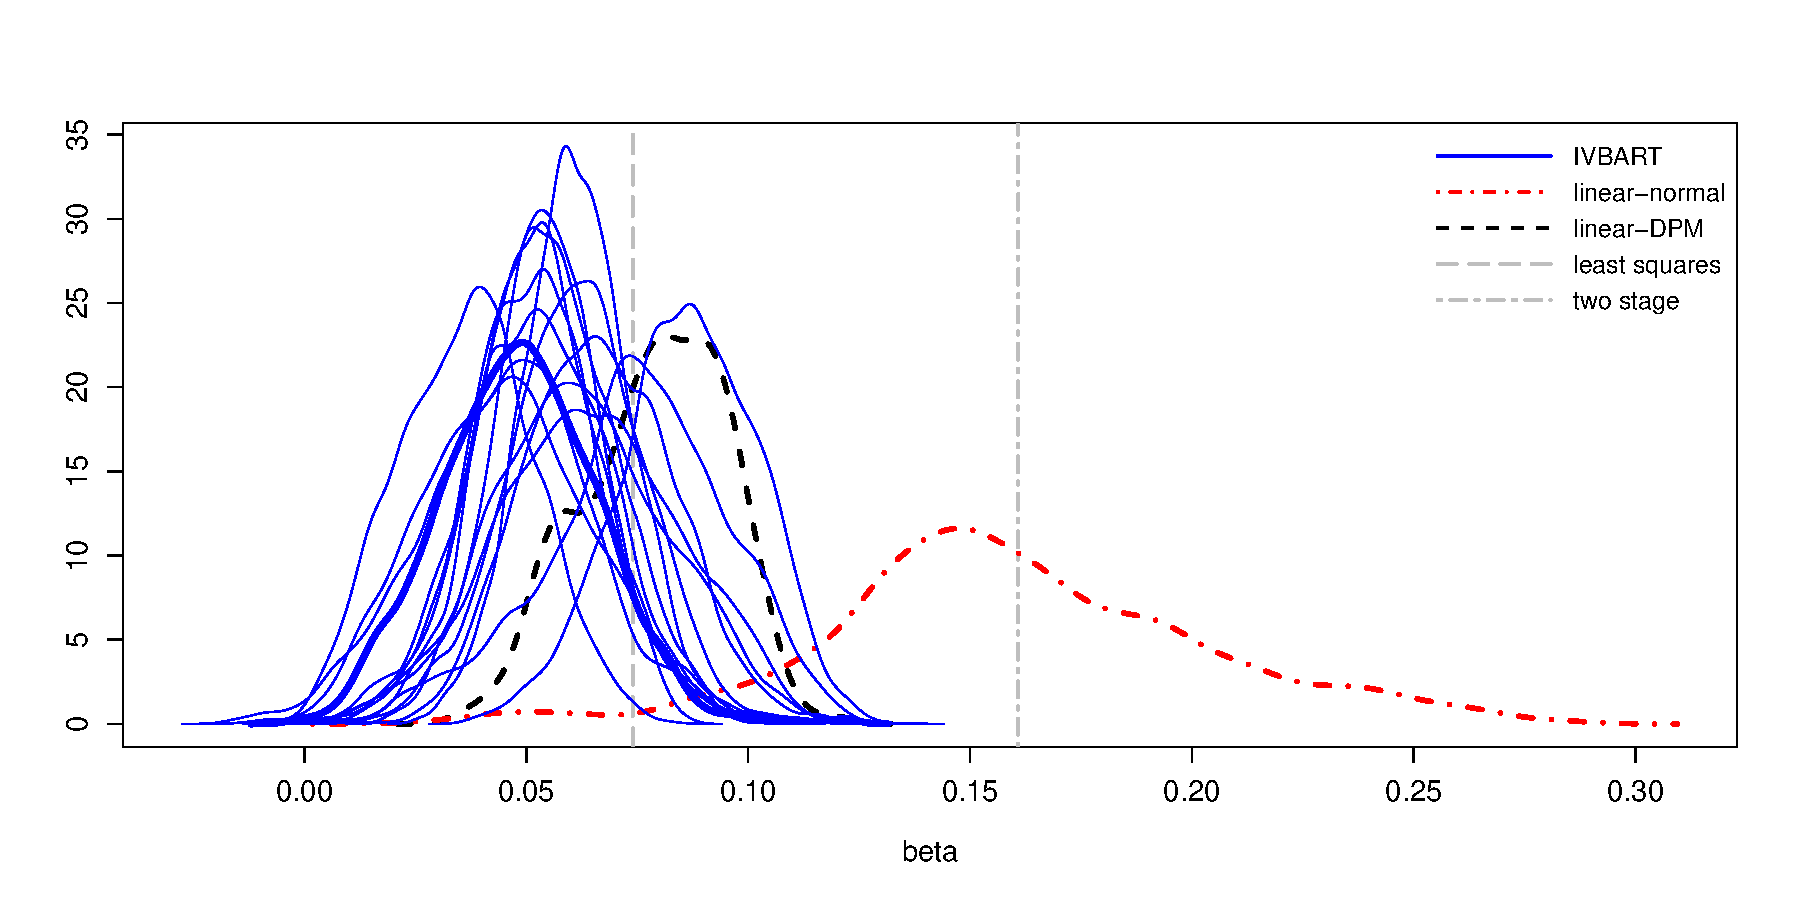
\includegraphics[scale=.6]{card-ivbart-2w-sens-1.pdf}}
\caption{%
Inference for $\beta$ for the Card data.
To assess prior sensitivity, we vary both $\sigma_f$ and $\sigma_g$ 
in (.8,1.0,1.2,1.4) giving 16 possible choices for the pair.
All 16 IVBART posteriors are drawn with a solid curve.
The thicker IVBART line is for the setting $(\sigma_f,\sigma_h) = (1.2,1.2)$.
Densities
for draws from the linear-normal (dot-dash line) and linear-DPM (dashed line) models are
also shown.
\label{fig:card-data-2w-sens-1}}
\end{figure}

\begin{figure}
\centerline{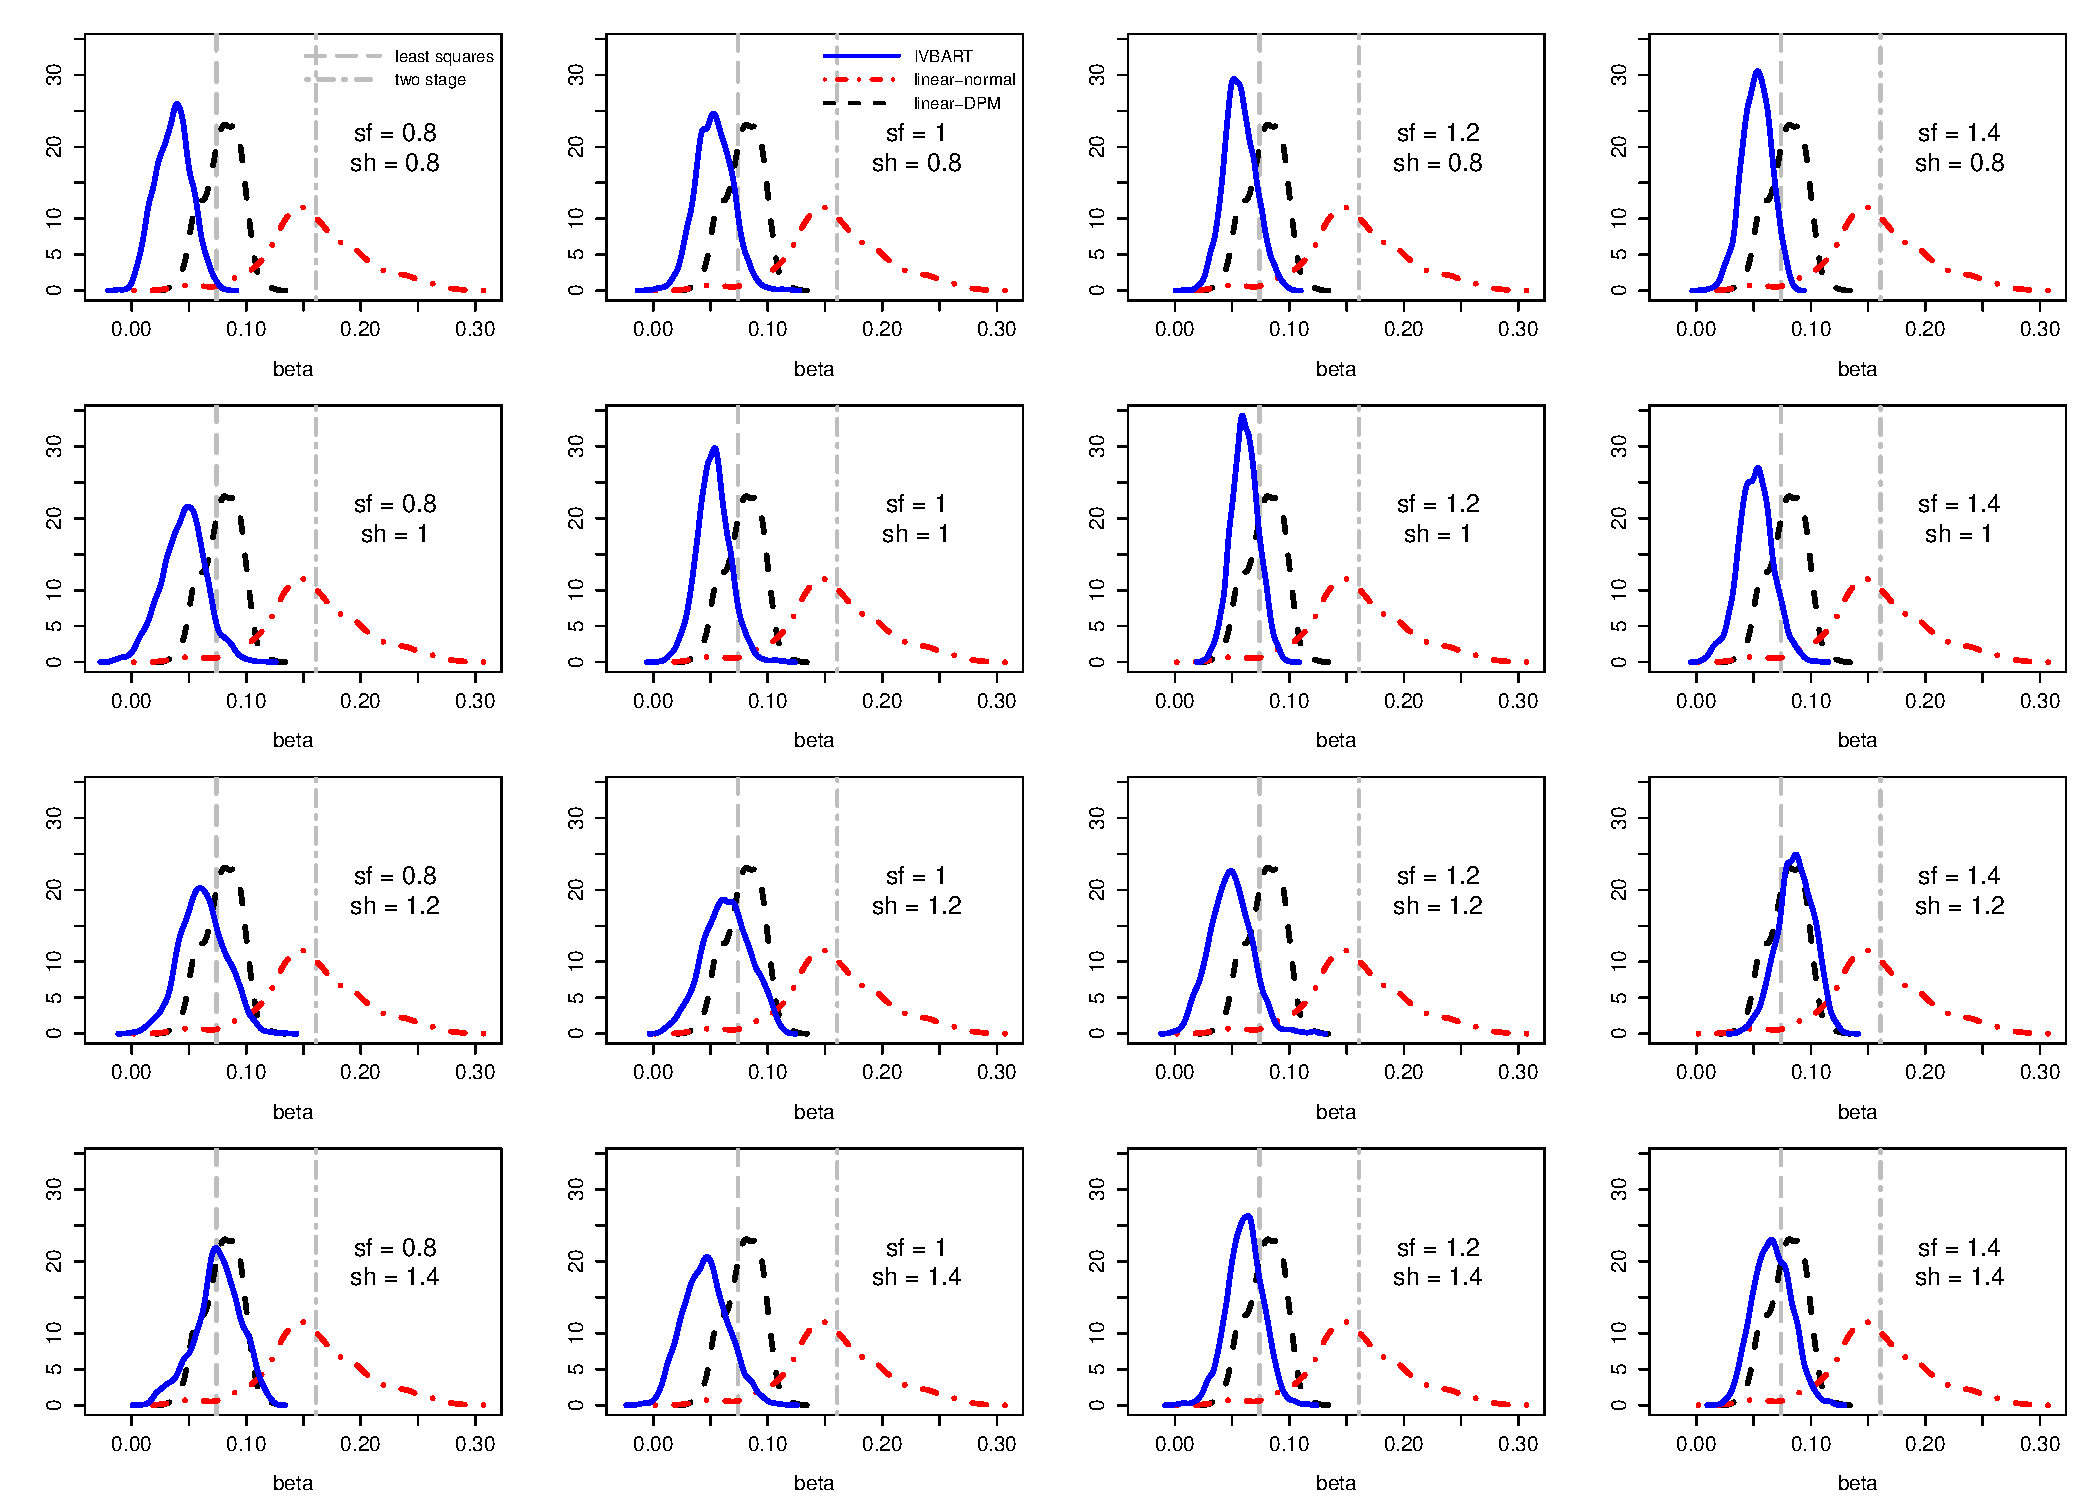
\includegraphics[scale=.5]{card-ivbart-2w-sens-4.pdf}}
\caption{%
Inference for $\beta$ from the Card data.
To assess prior sensitivity, we vary both $\sigma_f$ and $\sigma_g$ in (.8,1.0,1.2,1.4) giving 16 possible choices for the pair.
Each plot in the figure corresponds to a different choice of $(\sigma_f,\sigma_h)$.
Densities for draws from the linear-normal (dot-dash line) and linear-DPM (dashed line) models are
also shown in each plot.
\label{fig:card-data-2w-sens-4}}
\end{figure}

%> ff = exp(4*c(.05,.08,.15))
%> print(ff)
%[1] 1.221403 1.377128 1.822119

%> dy = c(.15, .08, .05)*4
%> dy
%[1] 0.60 0.32 0.20
%> exp(dy)
%[1] 1.822119 1.377128 1.221403

To quickly get a rough sense of the practical difference in the inferences show in Figure~\ref{fig:card-data-2w-sens-1},
we can say that according to the linear-normal, linear-DPM, and IVBART models, $\beta$ could be about .15, .08, or .05.
A change of 4 more years of schooling would then change y=log wage by .6, .32, and .2.
If we exponentiate these amounts, we get 1.8, 1.38, and 1.22 for the ratio of the wage level with and without the four years schooling.
All of these amounts are quite different from one as a practical matter and a 38\% increase in wages is quite a bit more than a 22\% increase.




